



Knowledge graphs are ubiquitous data structure which are used to store really world entities (e.g., {\tt Alan Turing}) and their relations ({\tt Alan Turing}, {\tt wasBornIn}, {\tt United Kingdom}).
Since the debut in 2012, several widely used knowledge graphs have been proposed, which include Yago, Wikidata, Freebase and so on.
Knowledge graph reasoning which aims to discover/explain existing knowledge or infer new knowledge from existing information in the knowledge graph has emerged as an important research direction over the last few years ~\cite{binet}.
%It is the mainstay of many applications, such as question answering ~\cite{}, recommender systems ~\cite{}, fact checking ~\cite{} and many more.





Despite the great achievement in both academia and industry,
most of the existing works on knowledge graph reasoning belong to the {\em point-wise} approaches, which perform reasoning w.r.t. {\em a single piece of clue} (e.g., a triple ~\cite{transE}, a multi-hop query ~\cite{binet}, a complex query graph ~\cite{lihui}). For example in fact checking, given {\em a claim} (e.g., represented as a triple of the knowledge graph), it decides whether the claim is authentic or falsified ~\cite{kgminer, KL}.
However, {\em comparative reasoning} (~\cite{kompare, prototype_liu}) is rarely studied.
Different from point-wise reasoning (or reasoning over knowledge graph).
{\em Comparative reasoning} over knowledge graph ~\cite{kompare} focuses on inferring commonality and/or inconsistency with respect to multiple pieces of clues (e.g., multiple claims about a news article), which is a new research direction over knowledge graphs and can be widely applied to other applications, e.g., fact checking.



Comparative reasoning has many unique advantages compared with point-wise (single claim) fact checking.
This is because in many real-world situations, e.g., multimodal fake news detection ~\cite{multimodal}, single claim fact checking alone is insufficient, while
comparative reasoning
offers a more complete picture w.r.t. the input clues,
which in turn helps the users discover the subtle patterns (e.g., inconsistency) that would be invisible by point-wise approaches. When we verify the two claims/triples at the same time, the result may be inconsistent even though each claim/triple itself is consistent if we evaluate it individually.
Figure ~\ref{inconsistency} gives an example to illustrate the power of comparative reasoning.
Suppose there is a multi-modal news article and we wish to verify its truthfulness. To this end, two query graphs are extracted from the given news, respectively. One query graph contains all the information from the text, and the other contains the information from the image. If we perform point-wise reasoning to check each of these two query graphs {\em separately}, both seem to be true. However, if we perform reasoning w.r.t. both query graphs simultaneously, and by {\em comparison}, we could discover the subtle inconsistency between them (i.e., the different air plane types, the difference in maximum flying distances). In addition, comparative reasoning can also be used in knowledge graph expansion, integration and completion ~\cite{kompare}.


In this paper, we address the problem of comparative reasoning.
We mainly focus on two problems: pairwise comparative reasoning and collective comparative reasoning. To be specific, we address two key challenges as follows.
We leverage graph neural network and graph kernel to reveal the commonality and inconsistency among input clues according to the information in the background knowledge graph.
We propose several different algorithms and demonstrate their effectiveness. A common building block of comparative reasoning is {\em knowledge segment}, which is a small connection subgraph of a given clue (e.g., a triple or part of it) to summarize its semantic context.
Based on that, we present core algorithms to enable both {\em pairwise} reasoning and {\em collective} reasoning.
The key idea is to use the structure and semantic information in knowledge segments to help discover vague contradictions.

The main contributions of the paper are
\begin{itemize} %\itemsep -1pt
    \item {\bf Problem Definition.} We introduce comparative reasoning over knowledge graphs, which complements and expands
    the existing point-wise reasoning capabilities.
    \item {\bf Algorithms.} We propose a family of comparative reasoning algorithms which can solve both pairwise comparative reasoning and collective comparative reasoning.
    \item {\bf Empirical Evaluations.} We perform extensive empirical evaluations to demonstrate the efficacy of our proposed methods.
\end{itemize}


The rest of the paper is organized as follows. Section ~\ref{problem_definition} introduces notations used in this paper and gives the problem definition.
Section ~\ref{ks_extractt} introduces how to extract the knowledge segment from the knowledge graph.
Section ~\ref{methods} proposes different methods to solve comparative reasoning problem.
The experiment results are presented in Section ~\ref{experiments}, and the related work is reviewed in Section ~\ref{related-work}. Finally, the paper is concluded in Section ~\ref{conclusion}.

\begin{figure*}[ht!]
\centering
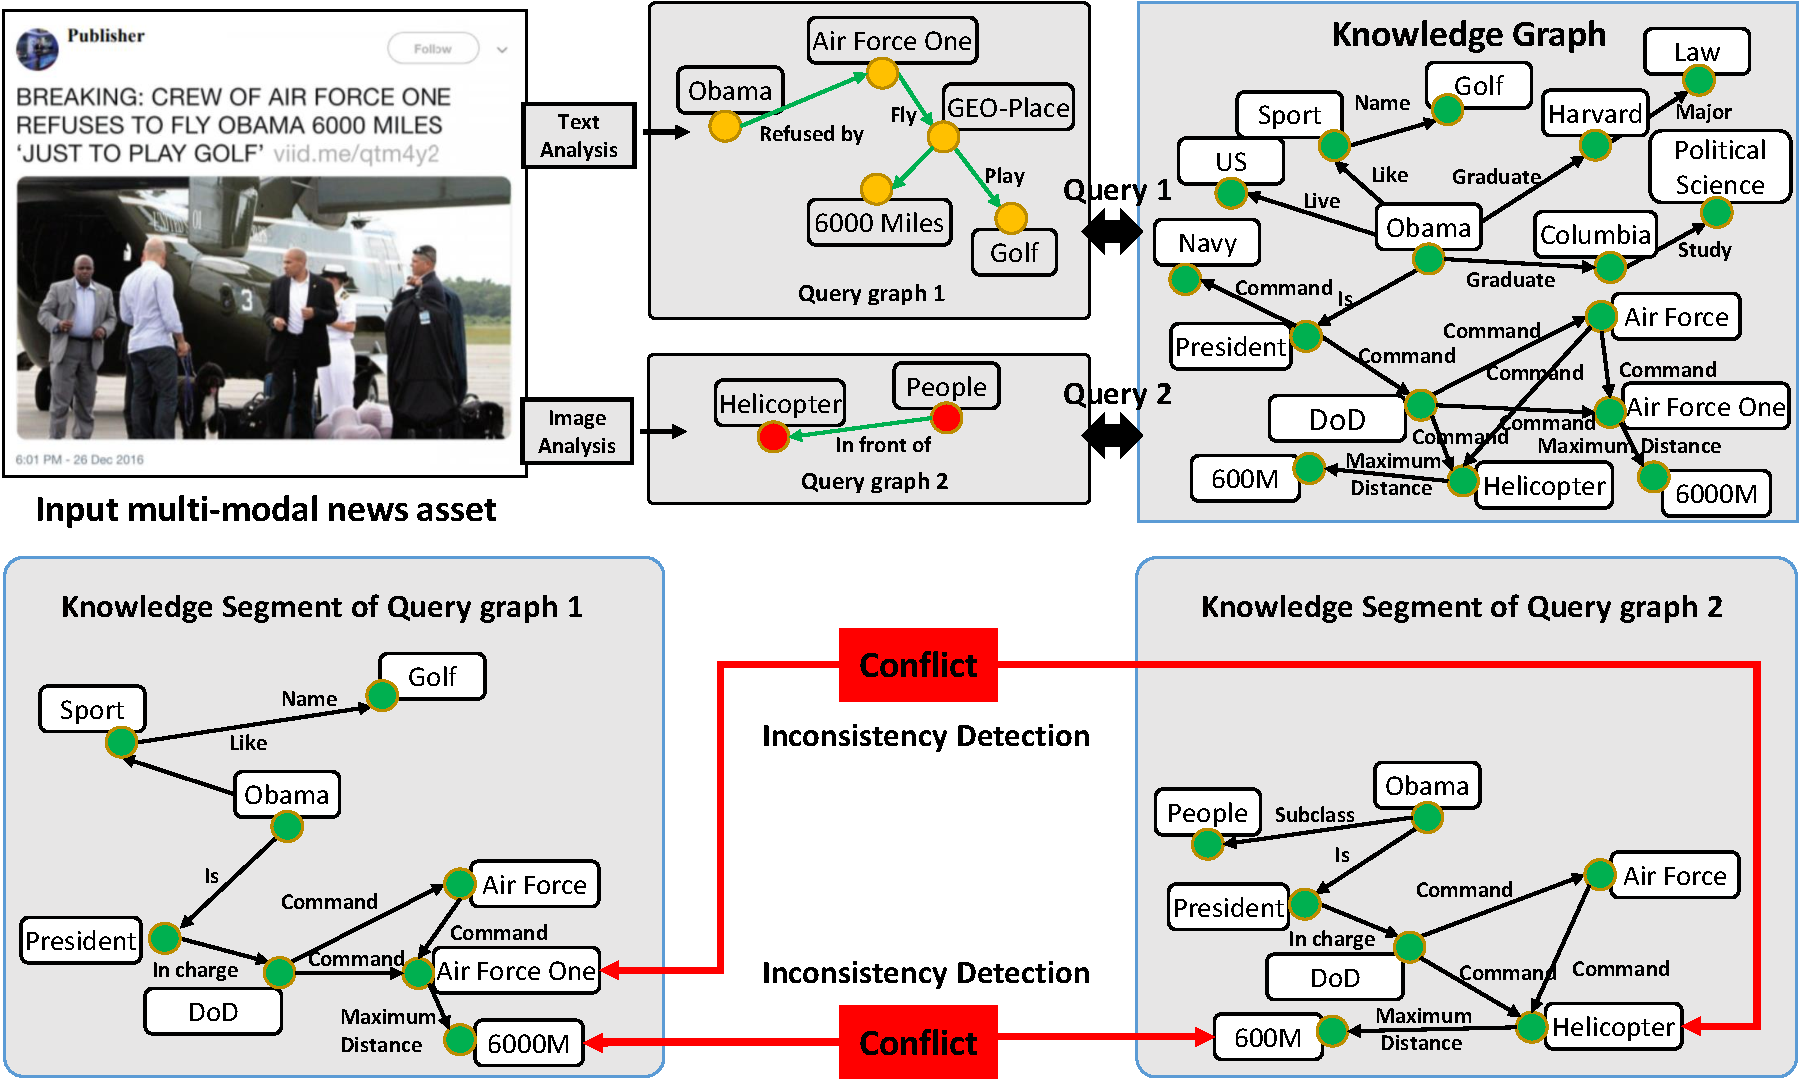
\includegraphics[width=0.8\textwidth]{submissions/logical-queries-uiuc/img/pdfresizer.pdf}
\caption{An illustrative example of using comparative reasoning for semantic inconsistency detection. Source of the image at the top-left: \cite{Cui2019SAMES}. The example is borrowed from ~\cite{kompare}.
}
\label{inconsistency}
\end{figure*}
